\documentclass[UTF8,nofonts,cs4size]{ctexrep}
\setCJKmainfont{SimSun} %中文为wqy 微米黑字体
%插入python代码使用的包,及其设定
\usepackage{color}
\usepackage{listings}
\usepackage{epstopdf}
\usepackage{graphicx}
\usepackage{multirow}
\usepackage{pythonhighlight}
\lstset{language=python}%这条命令可以让LaTeX排版时将C键字突出显示
\lstset{breaklines}%这条命令可以让LaTeX自动将长的代码行换行排版
\lstset{extendedchars=false}%这一条命令可以解决代码跨页时,章节标题,页眉等汉字不显示的问题

\lstset{
  language=python,
  keywordstyle=\color{blue},
  numbers=left,
  basicstyle=\ttfamily,
  frame=leftline,
  breaklines=true,
%  texcl=true,
%  backgroundcolor=\color{green!69!yellow!30!}
}

% 设定页边距
\usepackage[top=2.5cm,bottom=2.5cm,left=2.5cm,right=2.5cm]{ geometry}
% 加载 ams 数学公式与数学字体宏包
\usepackage{amsmath, amsfonts}
\usepackage{indentfirst}
\usepackage{graphicx}
%设置首行缩进
\usepackage{indentfirst}
\setlength{\parindent}{2em }
\setlength{\parskip}{0pt }
%段前段后距离设置
\CTEXsetup[beforeskip=0ex]{paragraph}
%页眉和页脚

\usepackage{fancyhdr}
\pagestyle{fancy}
\lhead{}
\chead{}
\rhead{}
\lfoot{}
\cfoot{\thepage}
\rfoot{}
\pagenumbering{Roman}

\renewcommand{\headrulewidth}{0pt}
\begin{document}

\begin{titlepage}

\newcommand{\HRule}{\rule{\linewidth}{0.5mm}} % Defines a new command for the horizontal lines, change thickness here

\center % Center everything on the page
 
%----------------------------------------------------------------------------------------
%	HEADING SECTIONS
%----------------------------------------------------------------------------------------

\textsc{\LARGE 安阳工学院}\\[1.5cm] % Name of your university/college
\textsc{\Large 密码学应用}\\[0.5cm] % Major heading such as course name


%----------------------------------------------------------------------------------------
%	TITLE SECTION
%----------------------------------------------------------------------------------------

\HRule \\[0.4cm]
{ \huge \bfseries RSA加密和解密算法的实现}\\[0.4cm] % Title of your document
\HRule \\[1.5cm]
 
%----------------------------------------------------------------------------------------
%	AUTHOR SECTION
%----------------------------------------------------------------------------------------

\begin{minipage}{0.4\textwidth}
\begin{flushleft}
\large
\emph{姓名}\textsc{: 申恒恒} \\
\emph{学号}\textsc{: 13031110141}\\
\emph{班级}\textsc{: 网络工程 13-1}\\
\emph{课程}\textsc{: 密码学应用}\\
\emph{老师}\textsc{: 齐万华} % Supervisor's Name
\end{flushleft}\end{minipage}\\[10cm]

% If you don't want a supervisor, uncomment the two lines below and remove the section above
%\Large \emph{Author:}\\
%John \textsc{Smith}\\[3cm] % Your name

%----------------------------------------------------------------------------------------
%	DATE SECTION
%----------------------------------------------------------------------------------------

\
\
\
{\large \today}\\[3cm] % Date, change the \today to a set date if you want to be precise

%----------------------------------------------------------------------------------------
%	LOGO SECTION
%----------------------------------------------------------------------------------------

%\includegraphics{Logo}\\[1cm] % Include a department/university logo - this will require the graphicx package
 
%----------------------------------------------------------------------------------------

\vfill % Fill the rest of the page with whitespace

\end{titlepage}
\title{\Large \bf 公钥密码RSA的实现 }
 
\author{申恒恒}
%设置中文章节的格式的字体
\CTEXsetup[format={\centering\zihao{3}}]{chapter}
\CTEXsetup[format={\bf\zihao{4}}]{section}
\CTEXsetup[format={\bf\zihao{-4}}]{subsection}

%设置中文摘要
\CTEXoptions[abstractname={\zihao{3}摘要}]
\begin{abstract}

传统的密码在密码分配和管理上是极为困难的,其中对于传统的对称密码来说,其中密钥配送很一个很大的问题,然而使用公钥密码可以解决上述密钥配送的问题。RSA作为公钥密码的代表\footnote{有时也称做非对称密码的代表},在公开密钥加密和电子商业中RSA被广泛使用。RSA由Ron River、Adi Shamir和Recnard Adleman在1978年共同发表了一种公钥密码加密算法\footnote{这三个个人于2002年授予计算机图灵奖}.本文主要阐述了公钥密码的基本原理、公钥密码的通信流程和其代表RSA算法的具体描述和其数学原理,RSA核心就是对极大整数做因数分解,对极大整数做因数分解的难度决定了RSA算法的可靠性。对一极大整数做因数分解越困难,RSA算法也就越可靠。但到现在到2016年为止,世界上还没有任何可靠的攻击RSA算法的方式。只要其钥匙的长度足够长,用RSA加密的信息实际上是不能被解破的。因此在了解了其背后的数学原理的基础上,利用Python语言实现了RSA加解密算法。\\
\indent 关键字:公钥密码、RSA算法、质因数分解、python语言实现
\end{abstract}


%设置目录的格式
\CTEXoptions[contentsname={\zihao{3}目\ 录}]
\tableofcontents



\pagenumbering{arabic}
\chapter*{前言}
\addcontentsline{toc}{chapter}{前言}
RSA作为计算机通信安全的基石,极为重要,有网络存在的地方就一定会有RSA的影子,RSA常常用于公钥密码和数字签名,RSA作为一种公钥密码算法,在公钥密码中,密钥常常分为加密密钥E和解密密钥D两种,发送方用E对消息进行加密,而接收方则用解密密钥D进行解密,而在传统的对称密码中,E和D是相同的,因此必须向接收者配送密钥。用于解密的密钥必须被配送到接收者手中,然而密钥的配送问题将在现实生活中确实很难解决的。\\
\indent 比如Alice在网络上认识了Bob,现在她想给Bob发一封E-mail,而且不想让别人知道邮件的内容,因此Alice决定使用对称密码进行加密,这样即便被窃听者Eve窃听到通信内容也没有问题.Alice将邮件内容进行加密生成了密文,当然现在如果将这封密文用邮件发送给Bob是不可以的,因为此时Bob是不可以直接对密文进行解密的。要使用对对称密码进行解密就必须使用和加密时相同的密钥才可以,也就是说只有同时将密钥发送给Bob,Bob才可以完成解密。\\
\indent  那么,此时采取将密文和密文通过E-mail发送给Bob,如果这样做,会导致窃听者Eve同时窃听到,这样的话,就相当于Bob一样的完成密文的解密并看到明文的内容,所以对于对称加密来说,解密密钥的配送是一个很大的挑战,但是对公钥密码来说,其完全不用考虑解密密钥的配送问题.\\
\indent  在公钥密码中,加密密钥和解密密钥是不同的,只要拥有加密密钥任何人都可以加密,但没有解密密钥是无法解密的,因此公钥密码相对对称加密又被称作做非对称密码,所以公钥密码其中一个重要的性质就是只有拥有解密密钥的人才能够进行解密。接受者事先将加密密钥发送给发送方,其中这个加密密钥被窃听者窃听也没有问题。发送方使用加密密钥对要发送的消息进行加密并将加密后的消息发送给接收方,而且只有拥有解密密钥的人才能够解密,这样以来就不需要将解密密钥配送给接收者,所以对于对称加密的密钥配送问题,公钥密码都可以解决,因此可以说公钥密码是密码学历史上的最伟大的发明。\\
\indent 了解了公钥密码的基本的作用后,那么在公钥密码系统中加密密钥又被称作公钥(pubic key),公钥密码一般是公开的,相对的,加密密钥是绝对不能公开的,这个加密密钥只能被自己使用,因此又被称作私钥(private key),私钥不可以被任何人知道,包括自己的通信对象。另外,公钥和私钥是一一对应的,一对公钥和私钥统称为密钥对。密钥对中的两个密钥之间具有非常密切的关系——数学上的关系——因此公钥和私钥是不能分别单独生成的。生活中常见的利用公钥密码的例子有银行卡,网络银行(网银),等等,其中公钥密码的私有密钥加密的文件只有公开密钥能解开.这一特点被用于PGP。\\
\indent 对于RSA作为公钥密码最成功的算法之一,在论文中会讨论公钥密码的基本流程和RSA密码的基本数学原理和加密、解密流程,同时给出加解密的具体操作,最后,在研究了RSA密码加解密流程基础之上。我使用python语言实现了一般的RSA加解密算法程序。在论文中阐述了主要的设计思路和实现方法。


\chapter{公钥密码}
\section{公钥密码的起源和概念}
公开密钥加密(英语:public-key cryptography,又译为公开密钥加密),也称为非对称加密(asymmetric cryptography),一种密码学算法类型,在这种密码学方法中,需要一对密钥,一个是私人密钥,另一个则是公开密钥。这两个密钥是数学相关,用某用户密钥加密后所得的信息,只能用该用户的解密密钥才能解密。如果知道了其中一个,并不能计算出另外一个。因此如果公开了一对密钥中的一个,并不会危害到另外一个的秘密性质。称公开的密钥为公钥;不公开的密钥为私钥。\\
\indent 该思想最早由瑞夫·墨克(Ralph C. Merkle)在1974年提出,之后在1976年。惠特菲尔德·迪菲(Whitfield Diffie)与马丁·赫尔曼(Martin Hellman)两位学者以单向函数与单向暗门函数为基础,为发讯与收讯的两方创建密钥。\\
\indent 如果加密密钥是公开的,这用于客户给私钥所有者上传加密的数据,这被称作为公开密钥加密(狭义)。例如,网络银行的客户发给银行网站的账户操作的加密数据。\\
\indent 如果解密密钥是公开的,用私钥加密的信息,可以用公钥对其解密,用于客户验证持有私钥一方发布的数据或文件是完整准确的,接收者由此可知这条信息确实来自于拥有私钥的某人,这被称作数字签名,公钥的形式就是数字证书。例如,从网上下载的安装程序,一般都带有程序制作者的数字签名,可以证明该程序的确是该作者(公司)发布的而不是第三方伪造的且未被篡改过(身份认证/验证)。\\
\indent 常见的公钥加密算法有:RSA、ElGamal、背包算法、Rabin(RSA的特例)、迪菲-赫尔曼密钥交换协议中的公钥加密算法、椭圆曲线加密算法(英语:Elliptic Curve Cryptography, ECC)。使用最广泛的是RSA算法(由发明者Rivest、Shmir和Adleman姓氏首字母缩写而来)是著名的公开金钥加密算法,ElGamal是另一种常用的非对称加密算法。
\section{公钥通信的流程}
下面简单描述一下公钥通信的基本流程,假设Alice要给Bob发送一条消息,Alice是发送者,Bob是接受者,而这一次窃听者Eve仍然窃听他们的通信内容。\\
\indent 在公钥密码通信中,通信是由接收者Bob启动的
\\ \indent\ \ (1) Bob生成一个包含公钥和私钥的密钥对 私钥由Bob自行妥善保管
\\ \indent\ \ (2) Bob将自己的公钥发送给Alice
\\ \indent\ \ (3) Alice使用Bob的公钥对消息加密
\\ \indent\ \ (4) Alice将密文将密文发送给Bob
\\

\begin{figure}{}
\centering
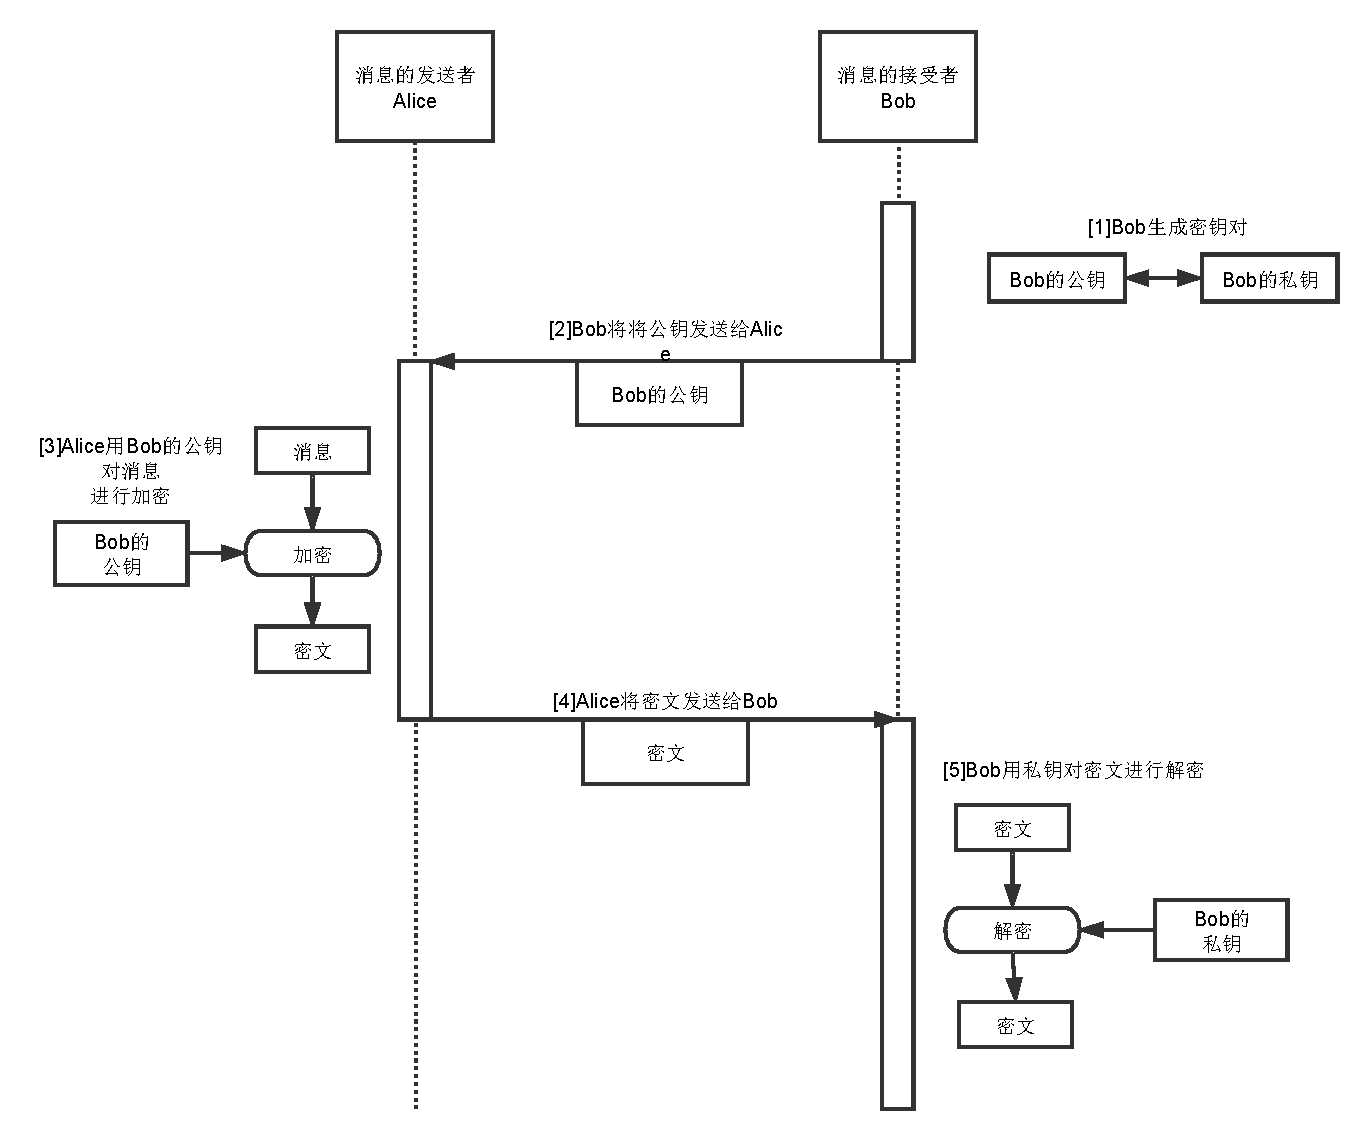
\includegraphics[scale = 0.7]{ss.pdf}
\caption{公钥通信流程图}
\end{figure}

\chapter{RSA算法}
RSA加密算法是一种非对称加密算法。在公开密钥加密和电子商业中RSA被广泛使用。RSA是1977年由罗纳德·李维斯特(Ron Rivest)、阿迪·萨莫尔(Adi Shamir)和伦纳德·阿德曼(Leonard Adleman)一起提出的。当时他们三人都在麻省理工学院工作。RSA就是他们三人姓氏开头字母拼在一起组成的。\\
\indent RSA可以被用于数字签名和公钥密码。下面介绍一下RSA的加解密算法和相关流程
\section{RSA 加密}
假设Bob想给Alice送一个消息m,他知道Alice产生的N和E。他使用起先与Alice约好的格式将m转换为一个小于N,且与N互质的整数n,比如他可以将每一个字转换为这个字的Unicode码,然后将这些数字连在一起组成一个数字。假如他的信息非常长的话,他可以将这个信息分为几段,然后将每一段转换为n。用下面这个公式他可以将n加密为c:
$$ c \equiv n^E \ (\mathrm{mod}\ N) $$
\indent 计算c并不复杂。Bob算出c后就可以将它传递给Alice。\\
\indent 在RSA中,明文、密钥和密文都是数字,在上面的公式里,E和N的组合就是公钥,即,任何人只要拿到这两个数字,就可以完成加密的操作。
\section{RSA 解密}
Alice得到Bob的消息c后就可以利用她的密钥D来解码。她可以用以下这个公式来将c转换为n:
$$ n \equiv c^D \ (\mathrm{mod}\ N) $$
\indent 得到n后,她可以将原来的信息m重新复原。\\
\indent 解码的原理是
$$ c^D \equiv n^{E \cdot D}\ (\mathrm{mod}\ N)$$
\indent 已知$ED \equiv 1 \pmod{r}$,即 $ED=1+h\varphi (N)$。 由欧拉定理得:
$$n^{ED} = n^{1 + h\varphi(N)} = n \left(n^{\varphi(N)}\right)^{h} \equiv n (1)^{h} \pmod{N} \equiv n \pmod{N}$$ 
\indent 注意在这里使用的N和RSA加密是的N是一样的,那么数字D和N的组合就是RSA的私钥.

\begin{table}[!hbp]
\centering
\begin{tabular}{|c|c|c|}
\hline
\hline

\multirow{2}{*}{密钥对} & 公钥 & 数E和数N \\
\cline{2-3}
 \multirow{2}{*}{} & 私钥& 数D和数N \\
\hline
\multicolumn{2}{|c|}{加密} & 密文 = 明文 $^E \ \mathrm{mod}\ N $\\
\hline
\multicolumn{2}{|c|}{解密} & 密文 = 明文 $^E \ \mathrm{mod}\ N $\\
\hline

\end{tabular}

\caption{RSA的加密和解密}
\end{table}

\begin{figure}{}
\centering
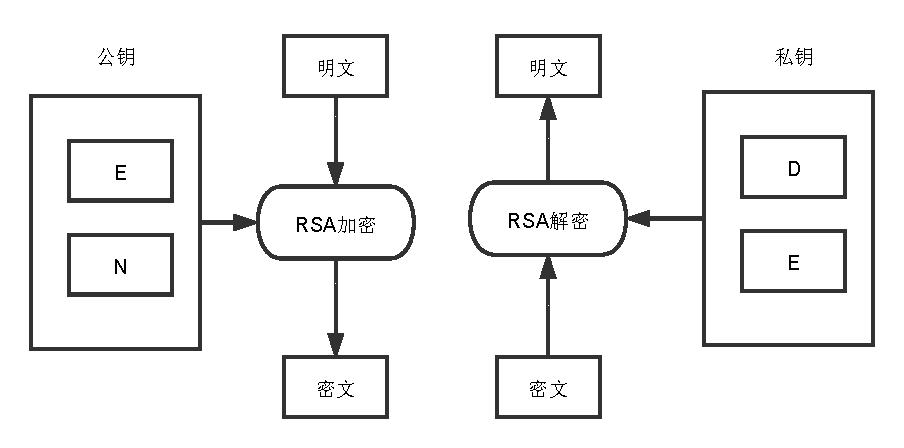
\includegraphics[scale = 0.8]{RSA.pdf}
\caption{RSA的加密和解密}
\end{figure}

\section{密钥对的生成}
由于E和N是公钥,D和N是私钥,因此求E、D和N这三个数就是生成密钥对,RSA生成密钥对的生成步骤如下:\\
\indent (1) 求N \\
\indent (2) 求L \\
\indent (3) 求E\\
\indent (4) 求D
\subsection{计算 N}
首先准备两个很大的质数 $p$ 和 $q$,它们的乘积就是 $N$。
$$N = p \cdot q $$
\indent 这里选择 $p = 29$, $q = 31$, 则 $N = p * q =$ 899。 

\subsection{计算 L}
$L$是在RSA的加密和解密过程中都不出现,只出现在生成密钥对的过程中。$L$是$p-1$和$q-1$的最小公倍数,用$lcm(X,Y)$来表示“$X$和$Y$的最小公倍数”,则$L$可以写作如下式子:
$$L = lcm(p-1,q-1)$$
\indent 在例子中,计算 $L = ( p - 1 ) \cdot ( q - 1 )=$ 840。

\subsection{计算 E}
E是一个比1大比$L$小的数,另外,$E$和$L$的最大公约数(gcd)必须为1,若用$gcd$表示$X$和$Y$的最大公约数,则E和L之间存在如下关系:
$$1 < E < L$$
$$gcd(E,L)  = 1$$

\indent 对于例子来说,这里选择 $E = 37$。
\subsection{计算 D}
数D是由E计算得到的,D、E和L之间必须具备如下关系:
$$1 < D < L $$
$$E \times D \ \mathrm{mod}\ L = 1 $$

\indent  在例子中用程序算的,算出来最小的 $D$ 就是 613\\
\indent 现在,得到了 $N$,$D$,$E$ ,把 $p$ 和 $q$ 扔掉,$(n, e)$作公钥,$(n, d)$作私钥,就可以执行 RSA 加密运算了。

\begin{figure}{}
\centering
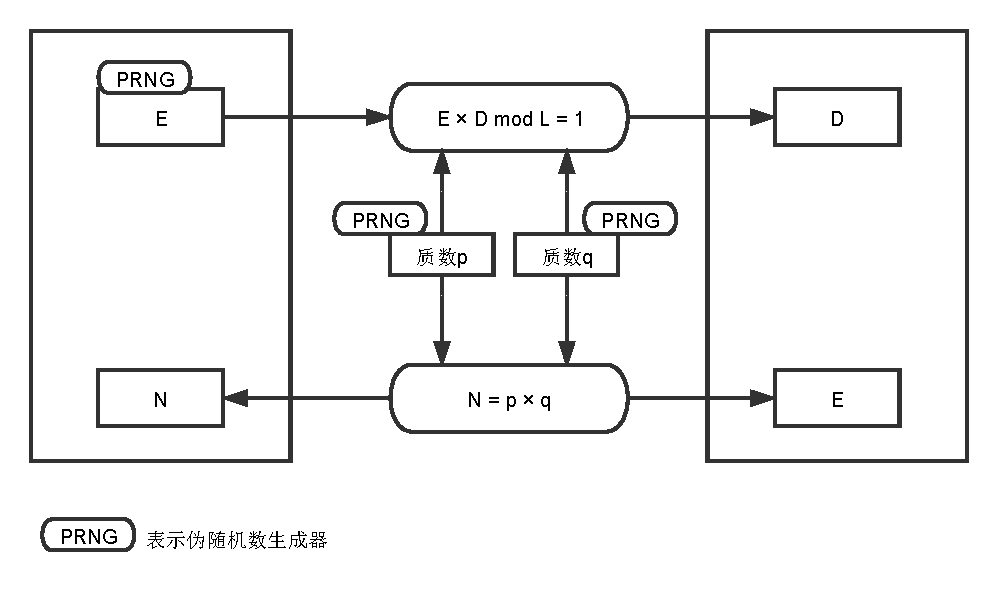
\includegraphics[scale = 0.8]{RSApair.pdf}
\caption{RSA密钥对生成过程}
\end{figure}


\chapter{RSA算法——Python实现}
为了实现一个简单的RSA加密和解密算法,可以使用模块化的设计方法,基于函数驱动的思想,将加解密算法中涉及到的各个过程(编码,加密编码,编码转化为密文或明文)抽象成一个个函数模块。然后通过各个函数之间的关系来涉及并实现游戏。通过前面中所介绍的RSA加密和解密的基本简单的过程实现。我们可以将所要实现的RSA加密描述如下:输入为明文字串格式,比如aaabbbbcccc,cccddeddfgggd等。然后根据前面描述的可知在RSA中,明文、密钥、密文均为数字,所以必须要对明文字串编码,编码为数字形式的列表这种数据结构,然后利用RSA的密文 = 明文 $^E\mathrm{\mod} N$求得密文。我们可以将所要实现的RSA解密描述如下:输入为密文的字串格式,比如aaabbbbcccc,cccddeddfgggd等。然后根据前面描述的可知在RSA中,明文、密钥、密文均为数字,所以必须要对密文字串编码,编码为数字形式的列表这种数据结构,然后利用RSA的明文 = 密文 $^D\mathrm{\mod} N$求得明文。
\section{概要描述}
阐述了RSA的基本原理和算法后,利用Python设计和实现一个RSA的加解密程序,在这里我将程序部署在Web上,利用Python的Flask框架结合Python程序作为后台加解密算法的引擎,以极为友好的方式展示出来。\\
\indent Python作为一门相当高级语言来说,具有简单易用,极为灵活的特点,本次RSA的实现主要根据RSA算法进行设计的,在$N$,$D$,$E$生成,往往会用到伪随机数生成器,但在项目中,只是验证性课题,只是对$N$,$E$,$D$进行了赋值,并没有密钥对的生成环节,换言之,已经将密钥对生成完毕,直接拿过来取加解密就可以,所以该程序主要实现了如下功能:\\
\indent (1) 在密钥对生成的基础上,如何利用$N$,$E$,$D$对数据(只支持字符串)进行加密和解密\\
\indent (2) 实现了米勒-拉宾素性测试

\section{整体设计}

加密和解密过程图如下
\begin{figure}{}
\centering
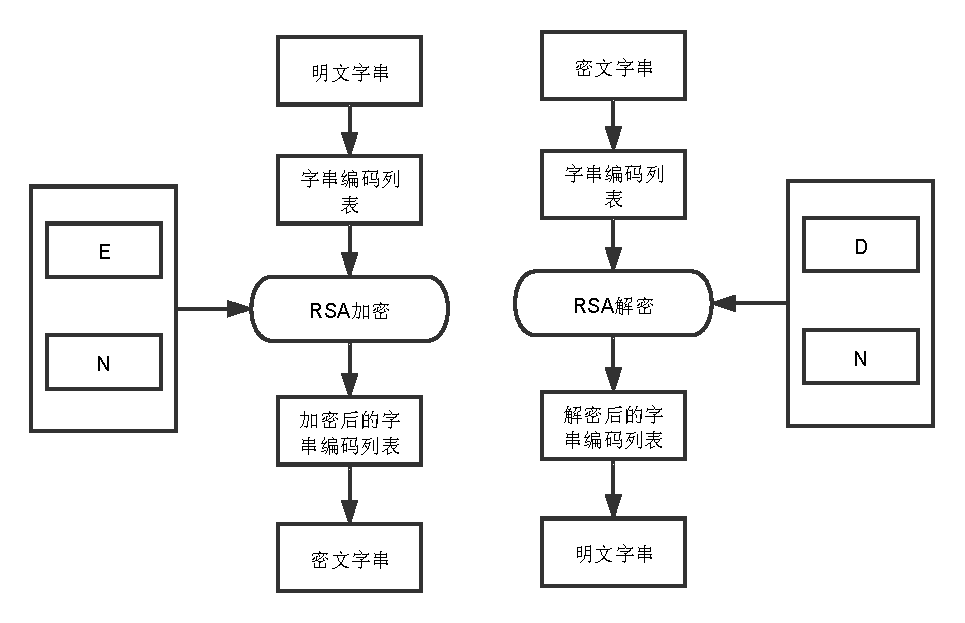
\includegraphics[scale=0.8]{encrypt-and-decrypt.pdf}
\caption{RSA加密和解密}
\end{figure}
\section{具体实现}
在程序中定义一个类RSA,该类实现了加密和解密函数及其辅助函数,具体如下:


\begin{python}
class RSA(object):
    def __init__(self):pass       
    def __chr_to_num(self, char):pass        
    def __num_to_chr(self, num):pass        
    def __text_to_array(self, text):pass        
    def __array_to_text(self, array):pass      
    def __array_to_cipher(self, array):pass     
    def __cipher_to_array(self, cipher):pass       
    def RSA_encrypt(self, text):pass    
    def RSA_decrypt(self, cipher):pass
  
\end{python}


\_\_init\_\_() 实现了RSA的初始化,在这里主要初始化了n,e,d,在RSA中分别表示大数N,公钥E,私钥D,由于前面算法给出的例子,这里我使用了手算指定N和公钥和私钥,并使他们符合上面的密钥对生成规则.根据前面的知识前面可以知道,n为两个大素数的乘积,这里p,q分别为29,31,那么e和d就可以计算出来。
例如,在程序中初始化了以下:
\begin{python}
def __init__(self):
        self.n = 29*31 
        self.e = 11
        self.d = 611

        self.__encryptnum = lambda m: calc_mod(m, self.e, self.n)
        self.__decryptnum = lambda c: calc_mod(c, self.d, self.n)
\end{python}

\indent 由于后期的加解密的需要,这里没有使用到伪随机数生成器来初始化p,q,E,有以下几个原因:\\
\indent (1)伪随机数生成器会导致后续的加解密的计算的时间的开销 \\
\indent (2)这里的目的我只是实现其RSA的加解密原理即可,后续的复杂的数学理论计算要求不高\\
\indent 另外\_\_encryptnum 和 \_\_decryptnum 利用了python lambda表达式表示的,通过\textit{calc\_mod()}函数来实现加解密编码后的数字的,表示对于每个“消息”来说,进行加密和解密操作,且这里指示的“消息”为数字。\\
\indent \textit{\_\_chr\_to\_num()} 实现了ascill码编码成十进位数字,同理 \textit{\_\_num\_to\_chr()} 实现了十进位数字编码为ascill码。程序如下:

\begin{python}
def __chr_to_num(self, char):
        if char == " ":
            return 0
        elif char == "\0":
            return 27
        else:
            return ord(char)-64

    def __num_to_chr(self, num):
        if num == 0:
            return " "
        elif num == 27:
            return "\0"
        else:
            return chr(num+64)
\end{python}

\indent 其中ord()函数和chr()函数(对于8位的ASCII字符串)的配对函数,ord()函数以一个字符(长度为1的字符串)作为参数,返回对应的ASCII数值,同理chr()函数用一个范围在range(256)内的(就是0~255)整数作参数,返回一个对应的字符。\\
\indent \textit{\_\_text\_to\_array()}和\textit{\_\_array\_to\_text()}分别实现了如下功能:\\
\indent (1)将明文字串变为编码列表\\
\indent (2)将编码列表变为明文字串\\
\indent 其中涉及到了python中的内建高级函数\textit{map()},又称为map\footnote{map/reduce的概念来自Google的那篇大名鼎鼎的论文“MapReduce: Simplified Data Processing on Large Clusters”,他们作为google搜索引擎的基础算法,也是当今构建大数据,分布式系统的核心算法和操作} 操作,\textit{map()}函数接收两个参数,一个是函数,一个是Iterable,map将传入的函数依次作用到序列的每个元素,并把结果作为新的Iterator返回\footnote{引用自廖雪峰官方网站:http://www.liaoxuefeng.com/wiki}。代码实现如下:
\begin{python}
def __text_to_array(self, text):
        array = []
        if len(text)%2 != 0:                                                    
            text += "\0"
        t = map(self.__chr_to_num, text)
        for item in izip(t[::2], t[1::2]):
            pre, after = tuple(item)
            array.append(pre*28+after)
        return array

    def __array_to_text(self, array):
        text = ""
        for num in array:
            pre = num//28
            after = num%28
            text += "".join(map(self.__num_to_chr, [pre, after]))
        return text
\end{python}

\indent \textit{\_\_array\_to\_cipher()} 和 \textit{\_\_cipher\_to\_array()}分别实现了编码列表变成了密文字串和将密文字串转化为编码列表,在这里主要利用了python中内建的base64模块,base64模块是用来作base64编码解码的。这种编码方式在电子邮件中是很常见。它可以把不能作为文本显示的二进制数据编码为可显示的文本信息。编码后的文本大小会增大1/3。在程序中分别使用了encodestring和decodestring方法,encodestring,decodestring作为base64模块的一组,它们专门用来编码和解码字符串,因为base64编码后的字符除了英文字母和数字外还有三个字符 + / =, 其中=只是为了补全编码后的字符数为4的整数,在程序中会看到每次加密后的密文后面会出现=。程序如下:

\begin{python}
def __array_to_cipher(self, array):
        text = ""
        for num in array:
            pre = num//28
            after = num%28
            text += "".join(map(chr, [pre, after]))
        return base64.encodestring(text)

    def __cipher_to_array(self, cipher):
        array = []
        t = map(ord, base64.decodestring(cipher))
        for item in izip(t[::2], t[1::2]):
            pre, after = tuple(item)
            array.append(pre*28+after)
        return array
\end{python}

\indent \textit{RSA\_encrypt()}函数是整合的方法,主要实现RSA加密功能,其通过传递字串类型的参数,首先利用\textit{\_\_text\_to\_array()}将ascill码字符串转化为编码列表类型,然后利用\textit{map()}操作对编码列表\footnote{其实列表数据结构就是一个Interable类型的数据结构,即迭代器,类似的还有字典,元祖等等}的每个元素(编码)进行加密操作,加密后编码列表通过\textit{\_\_array\_to\_cipher}方法转化为密文。具体程序如下:
\begin{python}
def RSA_encrypt(self, text):
        text_array = self.__text_to_array(text)
        cipher_array = map(self.__encryptnum, text_array)
        cipher = self.__array_to_cipher(cipher_array)
        return cipher

\end{python}

\indent \textit{RSA\_decrypt()}函数同样也是整合的方法,主要实现RSA解密功能,其通过传递字串(密文)类型的参数,首先利用\textit{\_\_cipher\_to\_array}方法将密文转化为编码列表 cipher\_array,然后利用\textit{map()}操作对编码列表cipher\_array 的每个元素(编码)进行解密操作,解密后编码列表再通过\textit{\_\_array\_to\_text}方法转化为明文。具体程序如下:
\begin{python}

    def RSA_decrypt(self, cipher):
        cipher_array = self.__cipher_to_array(cipher)
        text_array = map(self.__decryptnum, cipher_array)
        text = self.__array_to_text(text_array)
        if text[-1] == "\0":
            return text[:-1]
        return text

\end{python}

\indent 最后,RSA类定义好了,通过\textit{RSA()}实例化一个RSA对象,然后传递参数,调用\textit{RSA\_encrypt}和\textit{RSA\_decrypt}对其加解密即可。

\section{测试环节}
要求:由于程序只对26个英文字母和空格进行了字符编码,所以输入要求须为26个字母和空格,程序只接受字串元素为字母和空格,其他将会给出警告.
\begin{figure}{}
\centering
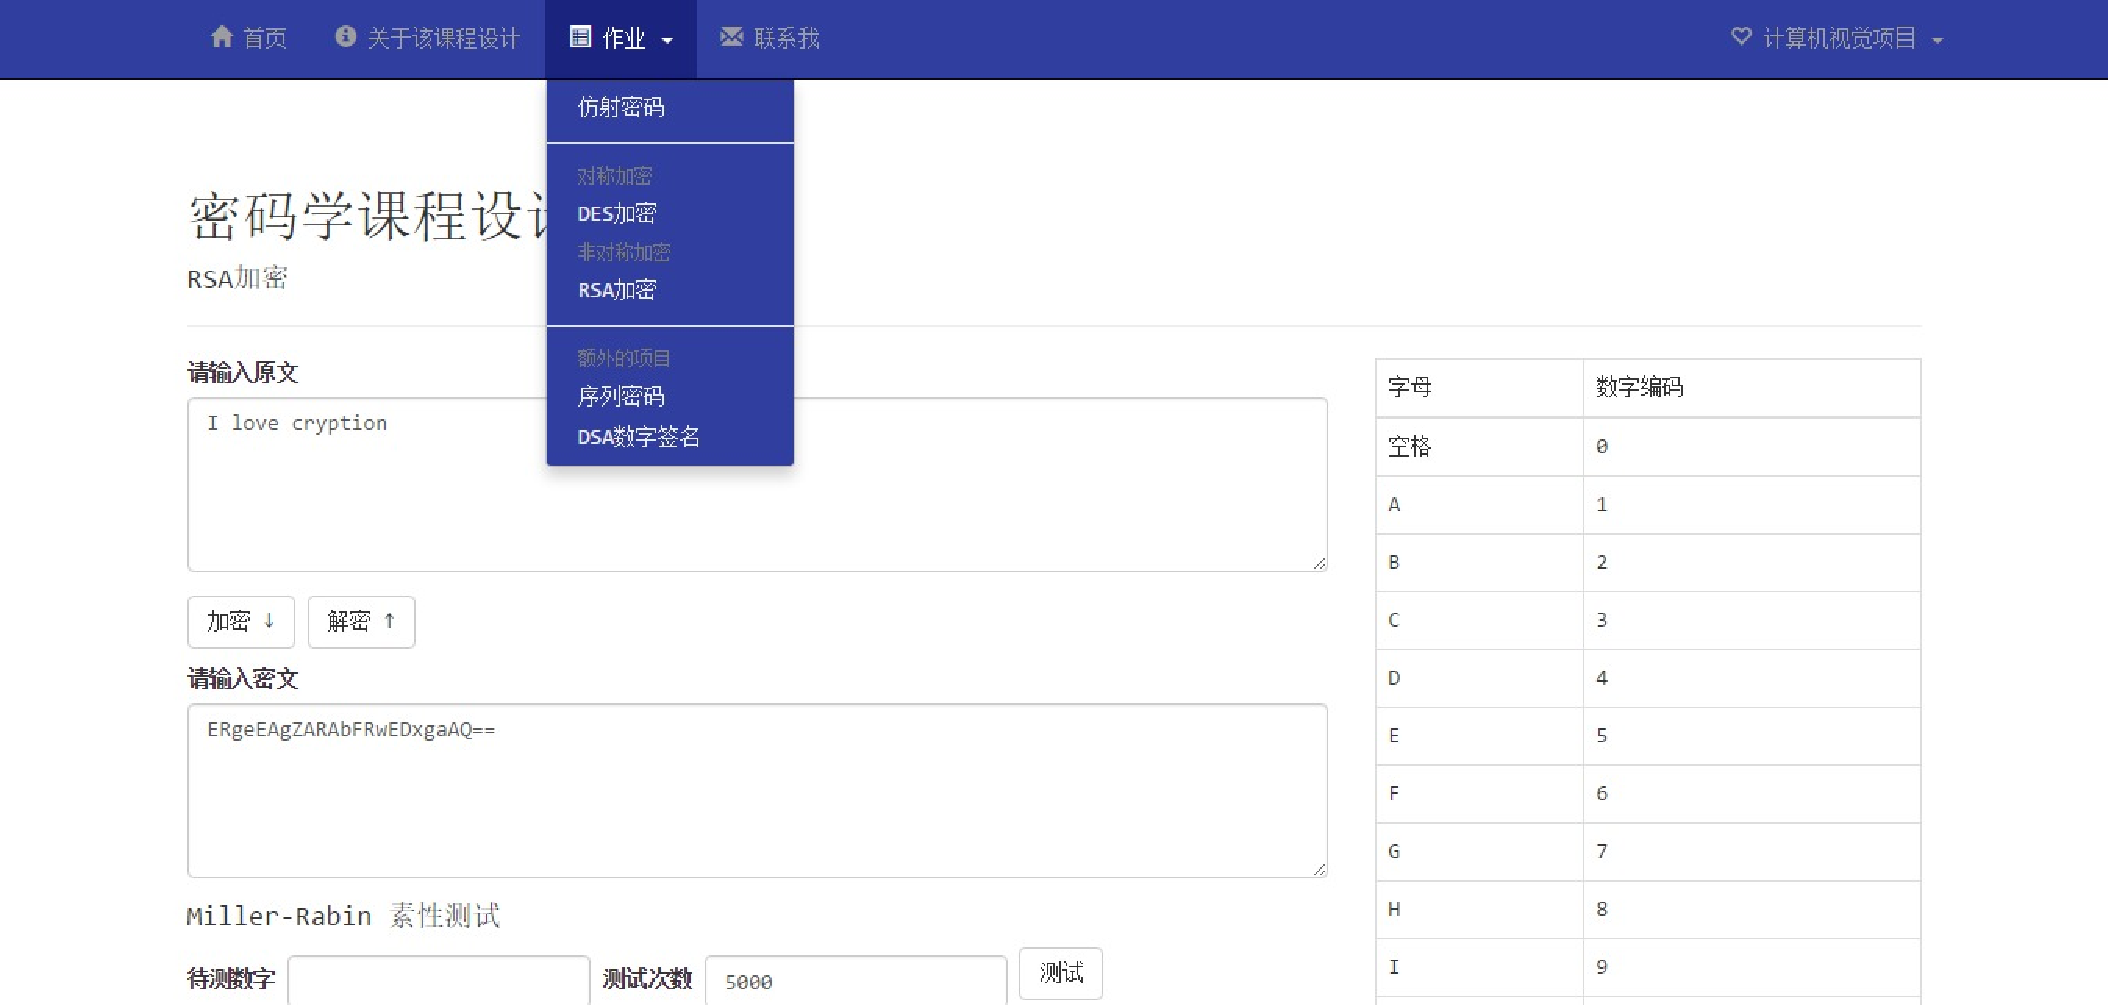
\includegraphics[scale=0.45]{snap.pdf}
\caption{RSA加密}
\end{figure}

\begin{figure}{}
\centering
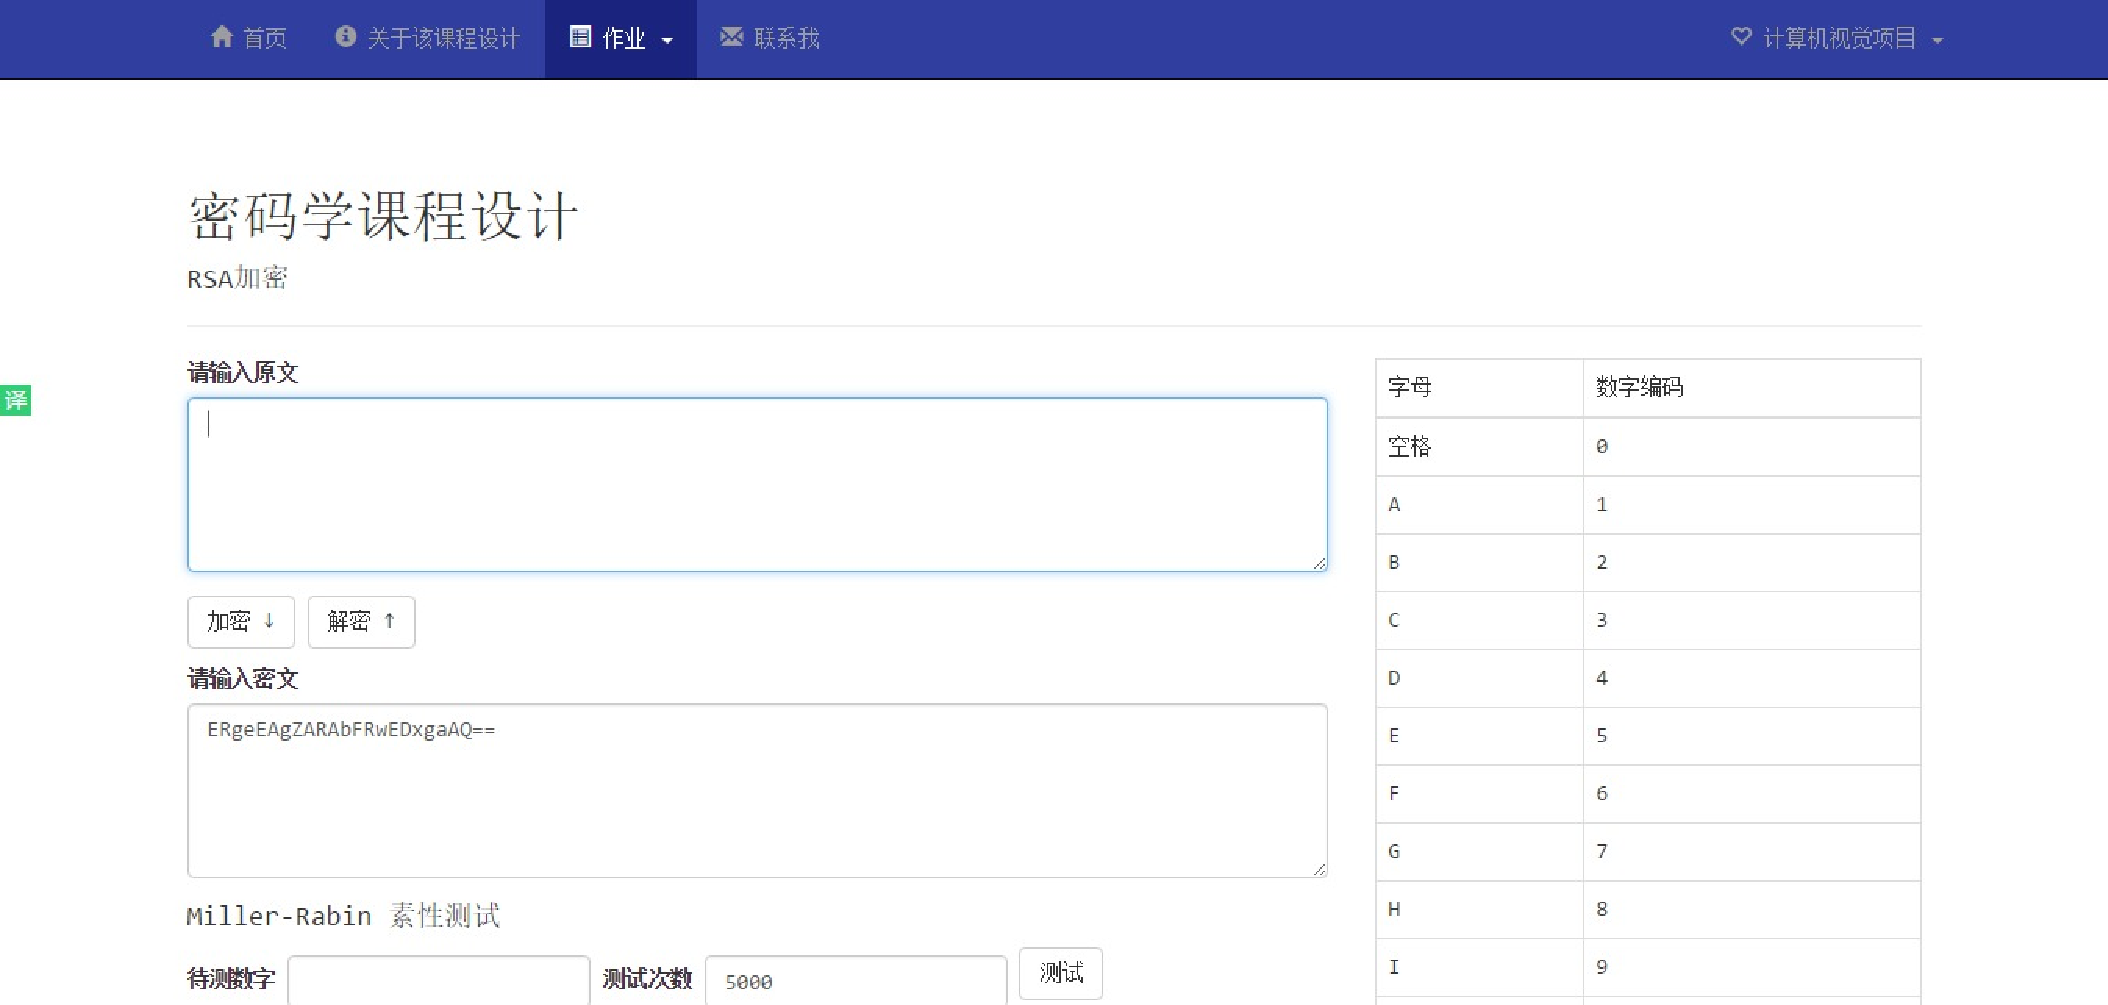
\includegraphics[scale=0.45]{ssB.pdf}
\caption{解密前密文}
\end{figure}

\begin{figure}{}
\centering
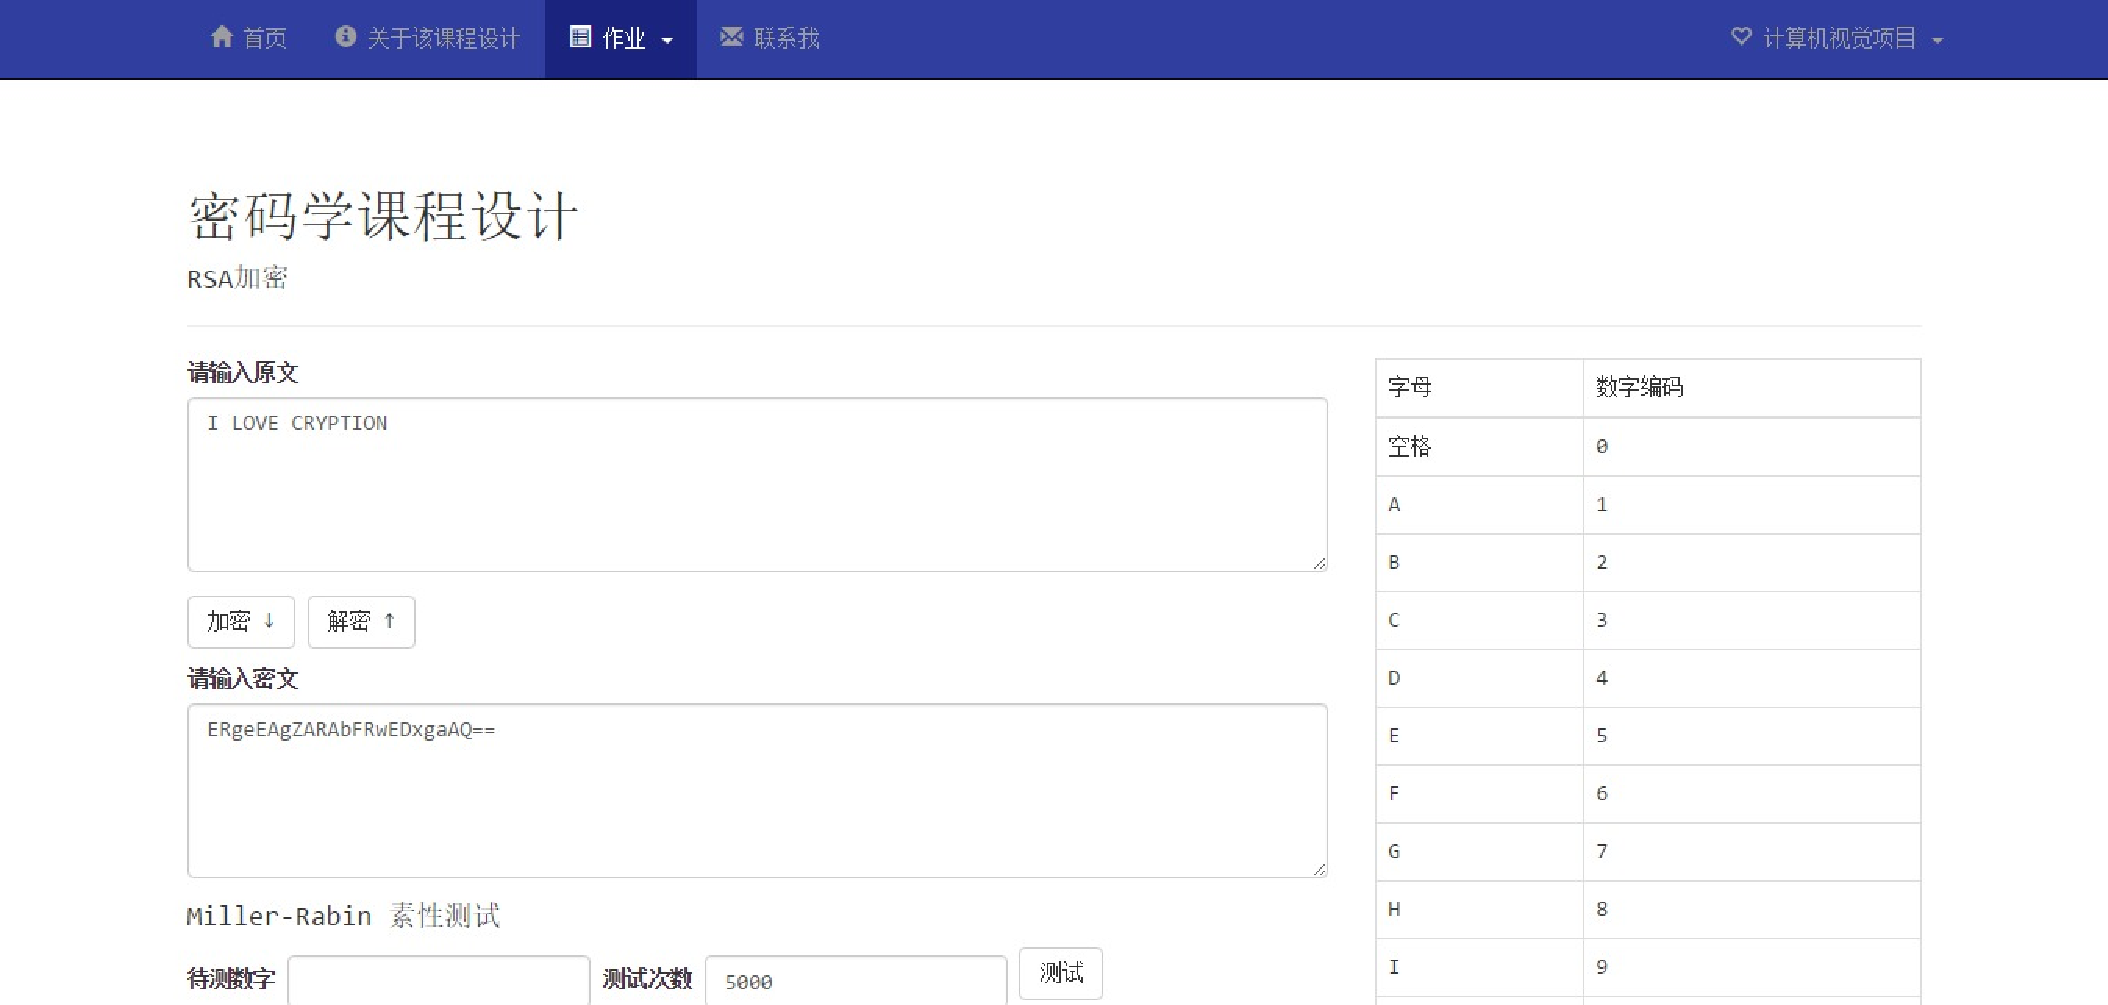
\includegraphics[scale=0.45]{ssA.pdf}
\caption{解密后}
\end{figure}

\begin{figure}{}
\centering
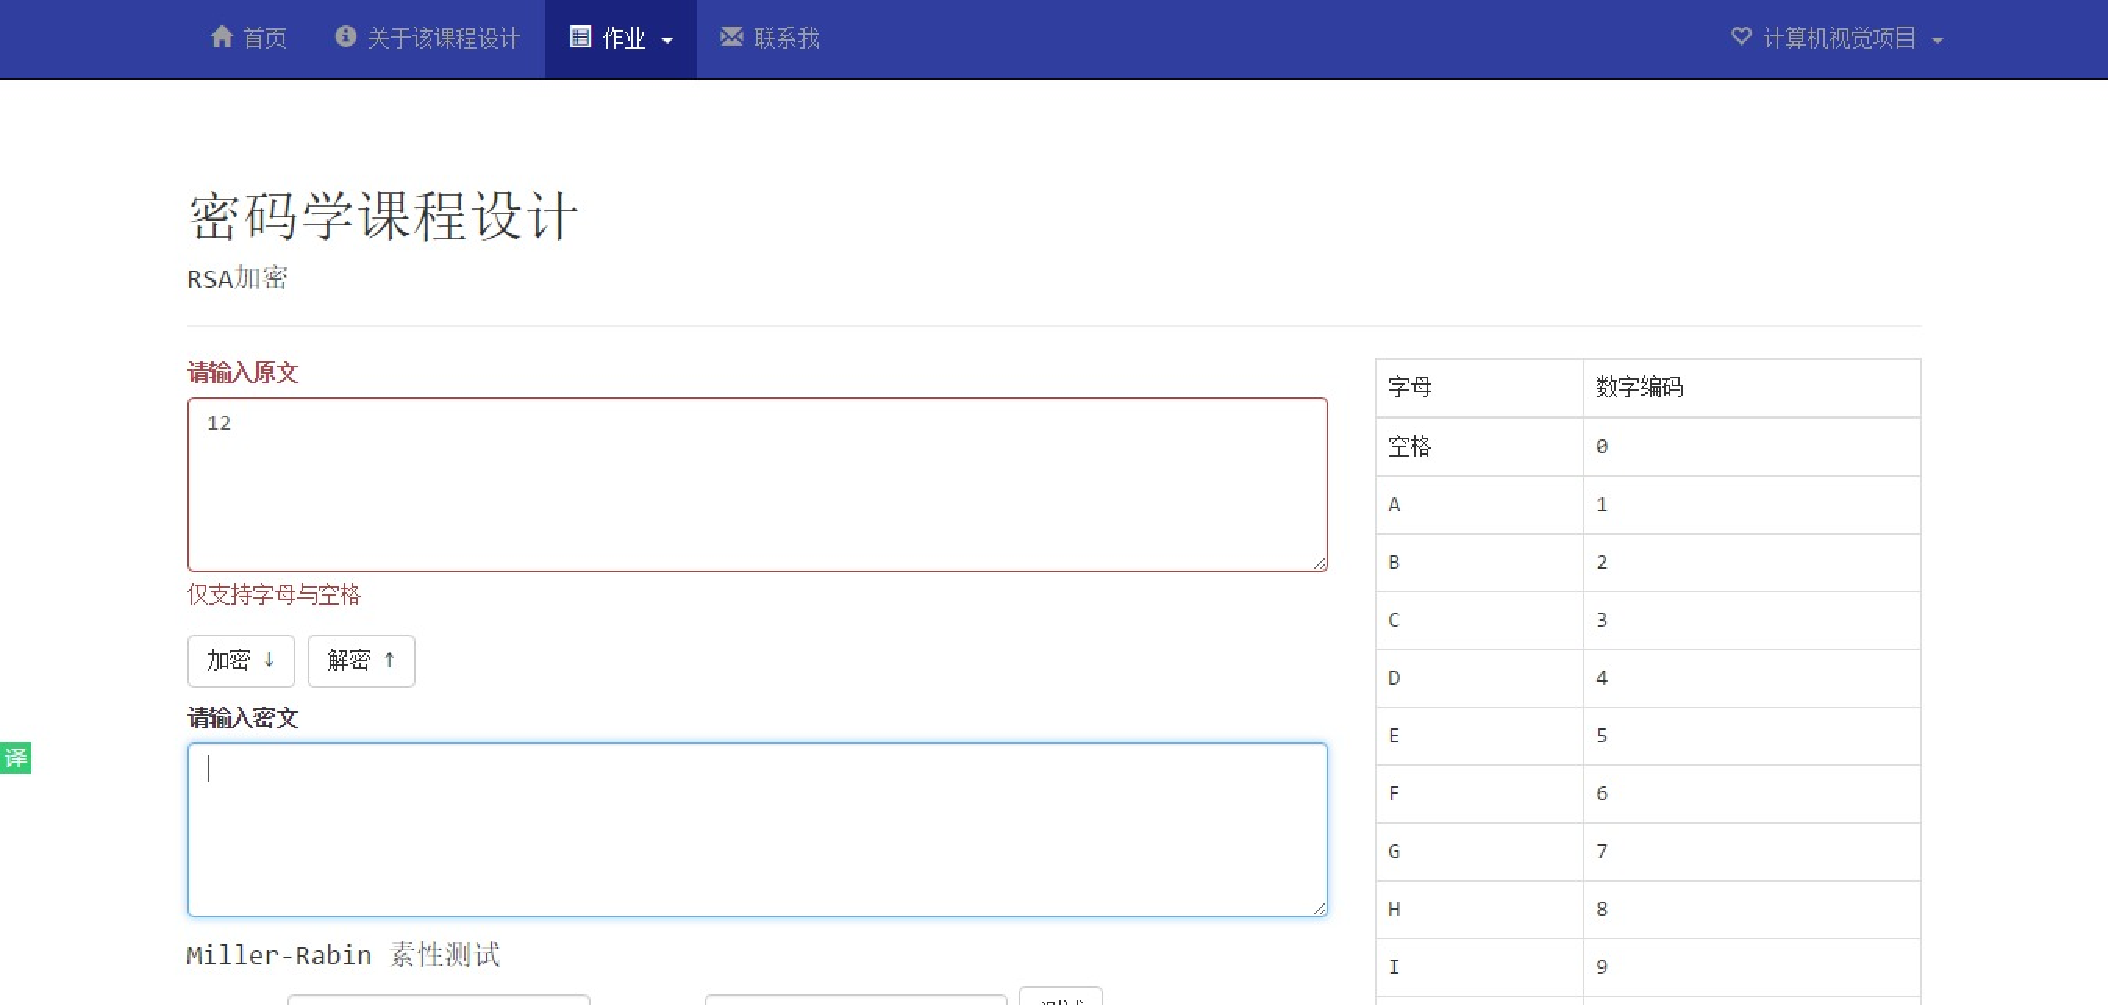
\includegraphics[scale=0.45]{ssC.pdf}
\caption{输入不符合规格给出警告}
\end{figure}

\begin{thebibliography}{99}
\addcontentsline{toc}{chapter}{参考文献}

\bibitem{computer}结城浩,图解密码技术,北京,人民邮电出版社,2015,98~123
\bibitem{1}朱文余,孙琦 计算机密码应用基础,北京,科学出版社,2003,93~97
\bibitem{3}Miguel Grinberg,Flask Web开发:基于Python的Web应用开发实战,北京,人民邮电出版社,2015,33~62

\end{thebibliography}
\appendix



\chapter{RSA源码}
\section*{RSA.py}
\begin{python}
# coding: utf-8
from utils import *
import base64
from itertools import izip

class RSA(object):
    def __init__(self):
        self.n = 29*31
        self.e = 11
        self.d = 611

        self.__encryptnum = lambda m: calc_mod(m, self.e, self.n)
        self.__decryptnum = lambda c: calc_mod(c, self.d, self.n)

    def __chr_to_num(self, char):
        if char == " ":
            return 0
        elif char == "\0":
            return 27
        else:
            return ord(char)-64

    def __num_to_chr(self, num):
        if num == 0:
            return " "
        elif num == 27:
            return "\0"
        else:
            return chr(num+64)

    def __text_to_array(self, text):
        array = []
        if len(text)%2 != 0:                                                
            text += "\0"

        t = map(self.__chr_to_num, text)
        for item in izip(t[::2], t[1::2]):
            pre, after = tuple(item)
            array.append(pre*28+after)

        return array

    def __array_to_text(self, array):
        text = ""
        for num in array:
            pre = num//28
            after = num%28
            text += "".join(map(self.__num_to_chr, [pre, after]))
        return text

    def __array_to_cipher(self, array):
        text = ""
        for num in array:
            pre = num//28
            after = num%28
            text += "".join(map(chr, [pre, after]))
        return base64.encodestring(text)

    def __cipher_to_array(self, cipher):
        array = []
        t = map(ord, base64.decodestring(cipher))
        for item in izip(t[::2], t[1::2]):
            pre, after = tuple(item)
            array.append(pre*28+after)
        return array

    def RSA_encrypt(self, text):
        text_array = self.__text_to_array(text)
        cipher_array = map(self.__encryptnum, text_array)
        cipher = self.__array_to_cipher(cipher_array)
        return cipher

    def RSA_decrypt(self, cipher):
        cipher_array = self.__cipher_to_array(cipher)
        text_array = map(self.__decryptnum, cipher_array)
        text = self.__array_to_text(text_array)
        if text[-1] == "\0":
            return text[:-1]
        return text

if __name__ == '__main__':
    rsa = RSA()
    a = "I LOVE YOU"
    s = rsa.RSA_encrypt(a)
    print s
    d = rsa.RSA_decrypt(s)
    print d

\end{python}



\section*{utils.py}
\begin{python}
# coding: utf-8
import timeit
import random

def calc_mod(x, r, n):
    """Calculate the value of x**r mod n"""
    a, b, c = x, r, 1
    while b != 0:
        while b%2 == 0:
            b = b/2
            a = a*a%n
        else:
            b = b-1
            c = (c*a)%n
    return c

def calc_reverse(m, n):
    """Calculate the value of m^(-1) mod n"""
    N = n
    m %= n
    m, n = n, m
    q = []
    while True:
        q.append(m//n)
        m, n = n, m%n
        if n == 1:
            break
    P, Q = [1, q[0]], [0, 1]
    for i in range(2, len(q)+1):
        P.append(P[i-2]+P[i-1]*q[i-1])
        Q.append(Q[i-2]+Q[i-1]*q[i-1])

    return (-1)**len(q)*P[-1]%N

def is_prime(n, k=5000):
    """Test whether n is a prime, repeat k times."""
    def mill_rab(n):
        b = 0
        while b%2 == 0:
            b = random.randint(2, n-1)     
        
        s, m = 0, n-1
        while m%2 == 0:                 
            m //= 2
            s += 1

        if calc_mod(b, m, n) == 1:
            return True
        else:
            for r in xrange(s):
                if calc_mod(b, 2**r*m, n) == n-1:
                    return True
        return False

    if n in [0, 1]:
        return False
    elif n == 2:
        return True
    for i in range(k):
        if not mill_rab(n):
            return False
    return True

if __name__ == '__main__':
    print(calc_reverse(11, 840))

\end{python}

\end{document}
